% ============================================================

\begin{frame}{Appendix --- Adjudication Geography and the Sample}
\hypertarget{app:geography}{}
\begin{columns}[T]

\begin{column}{0.60\textwidth}
  \vspace{-4pt}
  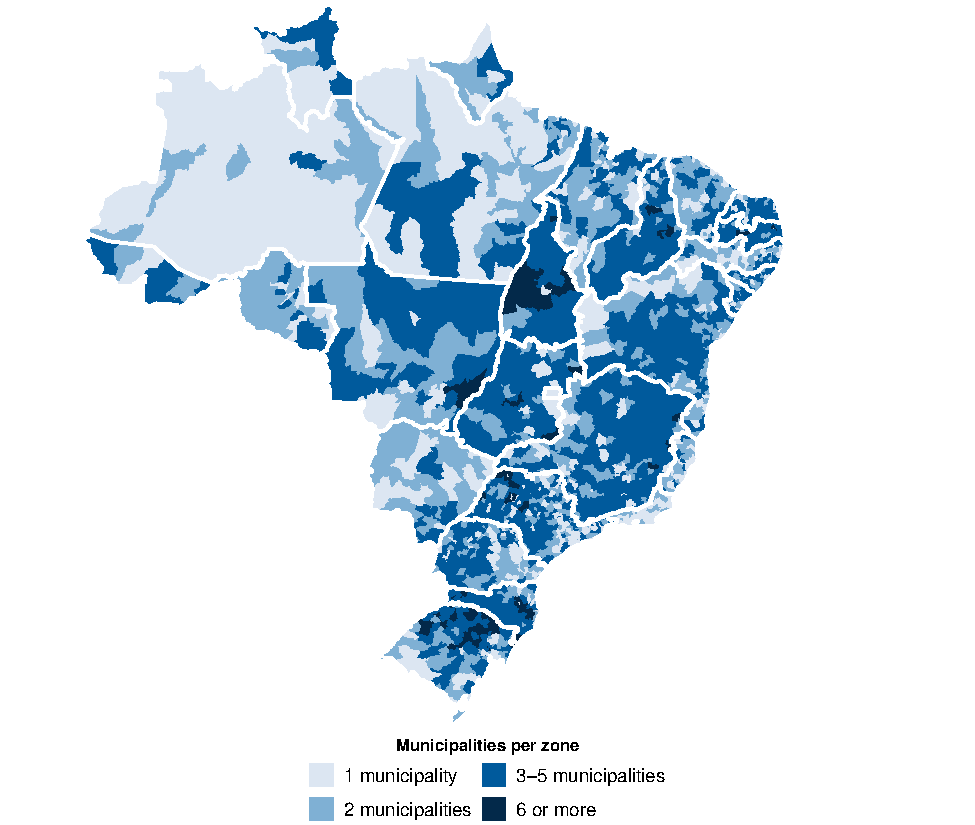
\includegraphics[width=\linewidth,height=0.55\textheight,keepaspectratio]{../figures/sample_map.pdf}
\end{column}

\begin{column}{0.38\textwidth}
  \vspace{4pt}
  \textbf{Adjudication geography}
  \smallskip

  \footnotesize
  \renewcommand{\arraystretch}{1.05}
  \begin{tabular}{lr}
    \toprule
    & \\[-6pt]
    Municipalities & \NMunisUniverse \\
    Electoral zones & \NZonesUniverse \\
    States (UF) & \NStatesUniverse \\
    Avg.\ munis per zone & \AvgMunisPerZone \\
    \bottomrule
  \end{tabular}

  \medskip
  \textbf{Zone size distribution}
  \smallskip

  \begin{tabular}{lrr}
    \toprule
    Munis per zone & Zones & Share \\
    \midrule
    1 & \ZoneDistOneN & \ZoneDistOnePct\% \\
    2 & \ZoneDistTwoN & \ZoneDistTwoPct\% \\
    3--5 & \ZoneDistThreeFiveN & \ZoneDistThreeFivePct\% \\
    6 or more & \ZoneDistSixN & \ZoneDistSixPct\% \\
    \bottomrule
  \end{tabular}

\end{column}

\end{columns}
\vspace{2pt}
\scriptsize
First-instance electoral cases are decided in the \emph{zona eleitoral} (\emph{ju\'izo eleitoral}), presided by a state judge. Each zone sits under one state electoral court (TRE), whose rulings bind every zone in the state, and the TSE sits above all. The decision locus is a three-tier hierarchy (zone $\subset$ state/TRE $\subset$ nation/TSE), and shocks to jurisprudence and enforcement diffuse down it. A zone holds \AvgMunisPerZone{} municipalities on average, many spanning several (table). We read each lawsuit's \textbf{munic\'ipio de origem} from the TSE SIG export (IBGE-matched for 99.99\% of filings) and analyze at the municipality level, while the adjudicating unit above it remains the \textbf{state/TRE}.\hfill\hyperlink{src:ejustice}{\beamerreturnbutton{Back}}
\end{frame}
